\chapter{Anexo III - Manuales de usuario e Instalación}

A modo de facilitar al lector el acceso y el uso de las herramientas empleadas en este \gls{tfm}, se dedicará este anexo a la creación de un manual de usuario. Se desarrollarán de forma detallada los procedimientos de instalación y configuración del software empleado, además de exponer su funcionamiento completo. De la misma forma, se incluirá la información necesaria para comprender conceptualmente los scripts que se han empleado con el fin de automatizar y optimizar el desarrollo de los casos prácticos.

% %%%%%%%%%%%%%%%%%%%%%%%%%%%%%%%%%%%%%%%%%%%%%%%%%%%%%%%%%%%%%%%%%%%%%%%%%%%%%%%%%%%%%%%%%



\section{Herramienta \acrshort{brite}}
\label{sec:manualbrite}

El objetivo de incluir esta sección es exponer al lector la información de instalación y configuración de la plataforma de generación de topologías de red \gls{brite}, descrita previamente en la Sección \ref{sec:brite}.

\subsection{Virtualización del sistema operativo Linux}
%%incluir una sección de virtualizacion de linux????? o esto va en condiciones?
Previamente a exponer los pasos de instalación del \gls{brite}, es preciso indicar que se ha empleado una máquina virtual con un sistema operativo Linux para soportar las funcionalidades de la herramienta. En este caso, se ha utilizado como plataforma VMWare\footnote{https://www.vmware.com/es/products.html} y una versión del sistema operativo Ubuntu 20.04.1 LTS como se puede visualizar en la Figura \ref{fig:ubuntu}.

\begin{figure}[h!]
    \centering
    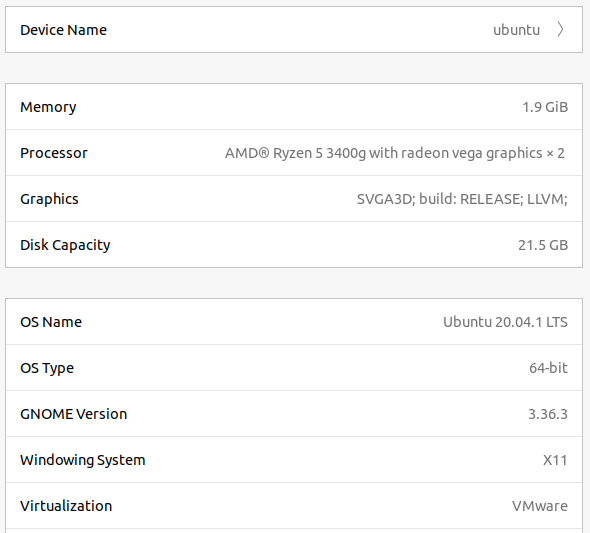
\includegraphics[width=0.75\textwidth]{img/anexos/ubuntu.PNG}
    \caption{Características del sistema operativo}
    \label{fig:ubuntu}
\end{figure}

\subsection{Compilación e instalación de \acrshort{brite}}

Para proceder a instalar la herramienta, se accede al repositorio del equipo de investigación NetIS de la \gls{uah}\footnote{https://github.com/NETSERV-UAH/BRITE} y se descarga y se descomprime el fichero .zip con todos los contenidos necesarios. Después, se realiza un \textit{make} desde el directorio raíz de la herramienta. Se pueden producir errores por la falta de paquetes \textit{g++} o \textit{openjdk++}, que se soluciona con los comandos dados en el Código \ref{paquetes}.

\begin{lstlisting}[language=bash, style=Consola, caption={Instalación de paquetes}, label={paquetes}]
sudo apt install g++
sudo apt install openjdk-11-jdk
\end{lstlisting}

\subsection{Ejecución de \acrshort{brite}}

Se puede ejecutar \gls{brite} mediante la interfaz gráfica (GUI) (ver Código \ref{lst:britegui}) o por comandos. En el caso de los comandos se da la posibilidad de utilizar los ejecutables programados en C++ o en Java (ver Código \ref{lst:ejecutar}), obteniéndose los mismos resultados a partir de una misma entrada.

\begin{lstlisting}[language=bash, style=Consola, caption={Ejecución de la interfaz gráfica de \gls{brite}}, label={lst:britegui}]
$./britegui &
\end{lstlisting}

\vspace{3mm}

\begin{lstlisting}[language=bash, style=Consola, caption={Ejecucion de \gls{brite} por la línea de comandos}, label={lst:ejecutar}]
$bin/brite <archivo de entrada .conf> <archivo de salida .brite> <seed_file>  
$C++/cppgen <archivo de entrada .conf> <archivo de salida .brite> <seed_file>
\end{lstlisting}

\vspace{3mm}

Como se especifica en el Código \ref{lst:ejecutar}, se requiere un archivo de configuración de entrada (.conf), en el cual se determinen los parámetros de la topología, y otro de salida, especificado en formato .brite. Como se ha expuesto en el Capítulo referente al Estado del Arte (ver Sección \ref{sec:brite_eje}), para facilitar el uso de \gls{brite} se aportan en el repositorio una serie de ficheros de Python y scripts dedicados a la automatización del proceso de creación de los ficheros de configuración y del tratamiento de la salida.





















%%%%%


%\cite{git}
%\cite{visual}